% Preamble: \pgfplotsset{width=15cm,compat=1.18}
\documentclass[a5paper]{article}
\usepackage{pgfplots}
\usepackage{pdflscape}
\usepackage[extreme]{savetrees}
\usepackage{xstring}
\pgfplotsset{compat=1.18}
\begin{document}
\thispagestyle{empty}
\begin{landscape}
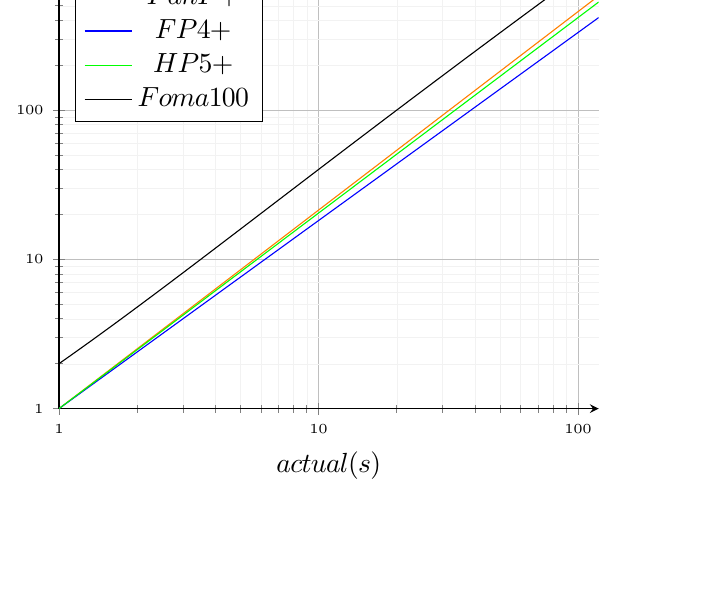
\begin{tikzpicture}
\centering
\usetikzlibrary{plotmarks}
\usepgfplotslibrary{units}
\begin{loglogaxis}[
    axis lines = left,
    xlabel = \(actual(s)\),
    ylabel = {\(measure(s)d\)},
    ticklabel style = {font=\tiny},
    grid=both,
    grid style={line width=.1pt, draw=gray!10},
    major grid style={line width=.2pt,draw=gray!50},
    legend pos=north west,
    log ticks with fixed point,
]
\addplot [
    domain=1:120,
    samples=100,
    color=orange,
]
{x ^ 1.33};
\addlegendentry{\(PanF+\)}

\addplot [
    domain=1:120,
    samples=100,
    color=blue,
]
{x ^ 1.26};
\addlegendentry{\(FP4+\)}

\addplot [
    domain=1:120,
    samples=100,
    color=green,
]
{x ^ 1.31};
\addlegendentry{\(HP5+\)}

\addplot [
    domain=1:120,
    samples=100,
    color=black,
]
{(log10 x)^2 + (log10 x) + 2) * x};
\addlegendentry{\(Foma100\)}

\end{loglogaxis}
\end{tikzpicture}
\end{landscape}
\end{document}
